\section{Method: \method{}}
\label{sec:method}

We propose Process-Aware Policy Optimization (\method{}), which integrates rubric-based process evaluation into GRPO through \emph{decoupled advantage normalization}. The key idea is to construct the advantage from independently normalized outcome and process components, preventing the reward hacking that arises from direct PRM integration while preserving fine-grained quality signals. Figure~\ref{fig:method_overview} provides an overview of the framework.

\begin{figure*}[t]
\centering
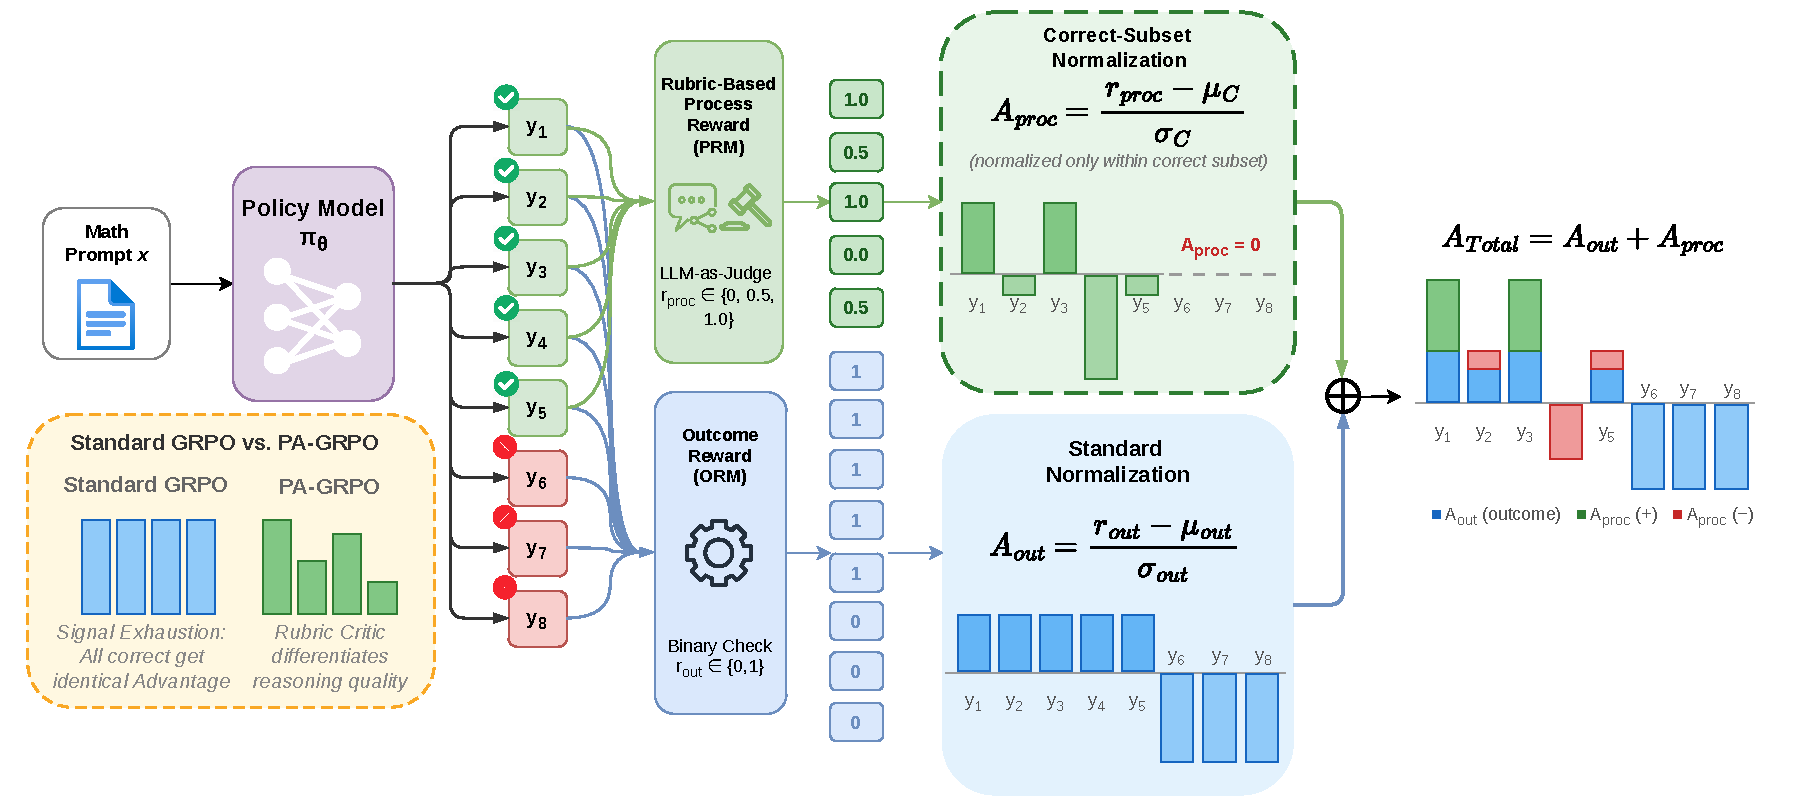
\includegraphics[width=\textwidth]{figures/fig_method_overview.pdf}
\caption{Overview of \method{}. Given a prompt, the policy generates $G$ responses. Each response is evaluated by two reward signals: an \textbf{outcome reward} (ORM, binary correctness) and a \textbf{process reward} (PRM, rubric-based quality, only for \textbf{correct responses}). The advantage is computed through \textbf{decoupled normalization}: $\aout$ is normalized over all responses via standard GRPO, while $\aproc$ is normalized exclusively among correct responses (\emph{correct-subset normalization}). The combined advantage $\atotal = \aout + \aproc$ provides both correctness direction and quality differentiation.}
\label{fig:method_overview}
\end{figure*}

\subsection{Dual Reward Signals}
\label{sec:reward-pipeline}

\method{} uses the ORM and rubric-based PRM described in \S\ref{sec:bg-rm} as two complementary reward signals: an outcome reward $r_i^{\text{out}} \in \{0, 1\}$ for answer correctness, and a process reward $r_i^{\text{proc}} \in \{0, 0.5, 1.0\}$ for reasoning quality. The PRM is only invoked for correct responses; incorrect responses are assigned $r_i^{\text{proc}} = 0$.

\subsection{Decoupled Advantage Normalization}
\label{sec:decoupled-adv}

Given a group of $G$ responses with rewards $\{(r_i^{\text{out}}, r_i^{\text{proc}})\}_{i=1}^G$, \method{} computes the advantage in three steps, as illustrated in Figure~\ref{fig:method_overview}:

\paragraph{Step 1: Outcome advantage $\aout$.} The outcome reward is normalized using standard GRPO group normalization:
\begin{equation}
\label{eq:a-out}
\aout[i] = \frac{r_i^{\text{out}} - \mu^{\text{out}}}{\max(\sigma^{\text{out}}, \epsilon)}
\end{equation}
where $\mu^{\text{out}}$ and $\sigma^{\text{out}}$ are the mean and standard deviation of $\{r_i^{\text{out}}\}_{i=1}^G$, and $\epsilon$ is a small constant for numerical stability. This component determines the ``correct vs.\ incorrect'' gradient direction, identical to standard GRPO.

\paragraph{Step 2: Process advantage $\aproc$ (correct-subset normalization).}
The process reward is normalized \emph{only among correct responses}:
\begin{equation}
\label{eq:a-proc}
\aproc[i] \!=\! \begin{cases}
\displaystyle\frac{r_i^{\text{proc}} - \mu_C^{\text{proc}}}{\max(\sigma_C^{\text{proc}}, \epsilon)} & \!\text{if } r_i^{\text{out}} \!=\! 1,\; |C| \!\geq\! 2 \\[6pt]
0 & \!\text{otherwise}
\end{cases}
\end{equation}
where $C = \{j : r_j^{\text{out}} = 1\}$ is the set of correct responses, and $\mu_C^{\text{proc}}, \sigma_C^{\text{proc}}$ are computed over $\{r_j^{\text{proc}}\}_{j \in C}$.

\paragraph{Step 3: Combined advantage.} The total advantage is the sum of the two components:
\begin{equation}
\label{eq:a-total}
\atotal[i] = \aout[i] + \aproc[i]
\end{equation}
Since both $\aout$ and $\aproc$ are independently normalized to zero mean and unit variance, they contribute on equal footing without requiring additional weighting.

\subsection{Design Rationale}
\label{sec:rationale}

The decoupled normalization addresses both failure modes identified in \S\ref{sec:problem}:

\paragraph{Quality differentiation without reward hacking.} Among correct responses, those with rigorous reasoning receive positive $\aproc$ and are reinforced, while those with sloppy or lucky reasoning receive negative $\aproc$ and are penalized. This quality signal is entirely absent in standard GRPO with binary ORM. Meanwhile, restricting normalization to the correct subset prevents incorrect responses from exploiting high PRM scores to gain positive $\aproc$, keeping the process signal decoupled from the outcome signal. We ablate this choice against full-group normalization in \S\ref{sec:ablation}.

\paragraph{Resolving signal exhaustion.} When all $G$ responses are correct, $\aout = 0$ for the entire group and standard GRPO produces no gradient. $\aproc$ remains active in this case, differentiating responses by reasoning quality and providing non-zero gradients that sustain learning. As shown in Figure~\ref{fig:signal_exhaustion}(a), this reduces the zero-advantage ratio from 69\% under ORM to 44\% under \method{}, maintaining a denser training signal throughout optimization. When fewer than two responses are correct, i.e., $|C| < 2$, $\aproc$ defaults to zero, gracefully reducing to standard GRPO.
